\subsection{Widoki}

Zostało stworzone kilka widoków:
\begin{itemize}
	\item \href{run:Sources/SQL/2. Widoki/014_Utworzenie_widoku_z_lista_wszystkich_najmow.sql}{\texttt{lista\_najmow} - Lista wszystkich najmów}
	\item \href{run:Sources/SQL/2. Widoki/015_Utworzenie_widoku_z_lista_popularnosci_obiektow.sql}{\texttt{lista\_popularnosci\_obiektow} - Lista obiektów wraz z ilością ich najmów}
	\item \href{run:Sources/SQL/2. Widoki/016_Utworzenie_widoku_z_lista_niewynajmowanych_obiektow.sql}{\texttt{lista\_niepopularnych\_obiektow} - Lista obiektów które nie zostały nigdy wynajęte}
\end{itemize}

\subsubsection{\texttt{lista\_najmow} - Lista wszystkich najmów}

Widok ten zwraca listę wszystkich najmów, wraz z następującymi polami:
\begin{itemize}
	\item nazwisko
	\item imie
	\item datę rozpoczecia najmu
	\item datę zakonczenia najmu
	\item nazwę wynajmowanego obiektu
	\item całkowity koszt najmu
\end{itemize}

\begin{figure}[h]
	\centering
    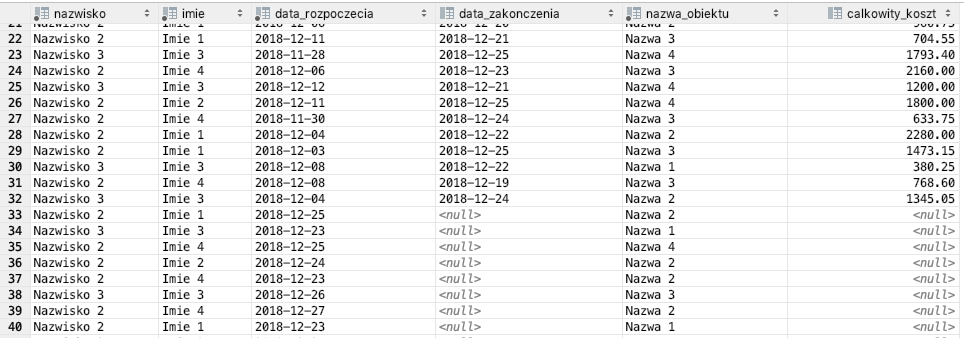
\includegraphics[width=0.9\textwidth]{lista_najmow}
	\caption{Wyświetlony widok \texttt{lista\_najmow}}
	\label{fig:lista_najmow}
\end{figure}



\subsubsection{\texttt{lista\_niepopularnych\_obiektow} - Lista obiektów które nie zostały nigdy wynajęte}

Widok ten zwraca listę obiektów które nie zostały nigdy, prze nikogo, wynajęte, wraz z następującymi polami:
\begin{itemize}
	\item nazwę obiektu
	\item adres obiektu
\end{itemize}

\begin{figure}[h]
	\centering
    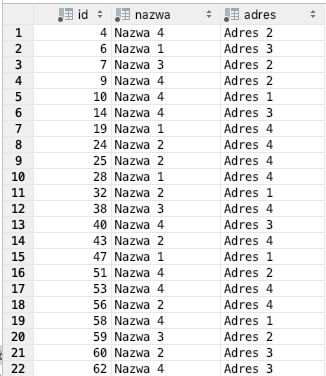
\includegraphics[width=0.4\textwidth]{lista_niepopularnych_obiektow}
	\caption{Wyświetlony widok \texttt{lista\_niepopularnych\_obiektow}}
	\label{fig:lista_niepopularnych_obiektow}
\end{figure}